\documentclass[a4paper,12pt]{article}
\usepackage[T2A]{fontenc}
\usepackage[utf8]{inputenc}
\usepackage[english,russian]{babel}
\usepackage{amsmath,amsfonts,amssymb,amsthm,mathtools}
\usepackage[margin=1in]{geometry}
\usepackage{amsmath, amsfonts, amssymb, amsthm, mathtools}
\usepackage{enumitem}
\usepackage{float}
\usepackage{graphicx}
\usepackage{tikz}
\graphicspath{ {images/} }
\usepackage{graphicx}
\graphicspath{{pictures/}}
\DeclareGraphicsExtensions{.pdf,.png,.jpg}

\newcommand{\N}{\mathbb{N}}
\newcommand{\Z}{\mathbb{Z}}

\newenvironment{theorem}[2][Theorem]{\begin{trivlist}
\item[\hskip \labelsep {\bfseries #1}\hskip \labelsep {\bfseries #2.}]}{\end{trivlist}}
\newenvironment{lemma}[2][Lemma]{\begin{trivlist}
\item[\hskip \labelsep {\bfseries #1}\hskip \labelsep {\bfseries #2.}]}{\end{trivlist}}
\newenvironment{exercise}[2][Exercise]{\begin{trivlist}
\item[\hskip \labelsep {\bfseries #1}\hskip \labelsep {\bfseries #2.}]}{\end{trivlist}}
\newenvironment{reflection}[2][Reflection]{\begin{trivlist}
\item[\hskip \labelsep {\bfseries #1}\hskip \labelsep {\bfseries #2.}]}{\end{trivlist}}
\newenvironment{proposition}[2][Proposition]{\begin{trivlist}
\item[\hskip \labelsep {\bfseries #1}\hskip \labelsep {\bfseries #2.}]}{\end{trivlist}}
\newenvironment{corollary}[2][Corollary]{\begin{trivlist}
\item[\hskip \labelsep {\bfseries #1}\hskip \labelsep {\bfseries #2.}]}{\end{trivlist}}
\author{Vyacheslav Gorchakov}
\title{PCA on higher orders.}
\date{2021}
\begin{document}
\maketitle
\newpage

\smallskip

\begin{center}
{\bf Motivation }
\end{center}

Principal component analysis (PCA) is a classical
statistic technique that has been applied to many fields, such
as knowledge representation, face recognition and image
compression. The objectives of PCA are to reduce the dimensionality of the dataset and identify new meaningful underlying variables. The key idea is to project the objects to an orthogonal subspace for their compact representations. It can be noted that in the classical 1D-PCA
the 2D data sample (e.g. image) must be initially converted
to a 1D vector form. The resulting sample vector will lead
to a high dimensional vector space. It is consequently difficult to evaluate the covariance matrix accurately when the sample vector is very long and the number of training samples is small. However, advances of PCA approach have been mostly limited to vector or matrix type data despite the fact that continued advances in information and sensing technology have been making large-scale, multi-modal, and multi-relational datasets evermore commonplace. Indeed, such multimodal data sets are now commonly encountered in a hugevariety of applications including chemometrics, hyperspectral imaging, high resolution videos, neuroimaging (EEG, fMRI), biometrics and social network analysis. When applied to these higher order data sets, standard vector and matrix models such as PCA have been shown to be inadequate at capturing the cross-couplings across the different modes and burdened
by the increasing storage and computational costs. Therefore, there is a growing need for PCA type methods that can learn from tensor data while respecting its inherent multi-modal structure for multilinear dimensionality reduction and subspace estimation.

\begin{center}
{\bf Theory }
\end{center}
Let $[n] = {1,2,...,n}$ for all $n \in \mathbb{N}$. A $d-mode$ or $dth-order$ tensor is simply a d-dimensional array of complex valued data $\mathbb{A} \in \mathbb{C}^{n_1 \times n_2 \times .. \times n_d}$ for given dimensions $n_1, ..., n_d \in \mathbb{N}$.

The \textit{vectorization} of $\mathbb{A} \in \mathbb{C}^{n_1 \times n_2 \times .. \times n_d}$ will always reshape $\mathbb{A}$ into a vector denoted by $a \in \mathbb{C}^{n_1 \cdot n_2 \cdot...n_d}$

\paragraph{The Standard Inner Product Space of $d$-mode Tensors.}

Let $\mathbb{A} \in \mathbb{C}^{n_1 \times n_2 \times .. \times n_d}$ and $\mathbb{B} \in \mathbb{C}^{n_1^{'} \times n_2^{'} \times .. \times n_d^{'}}$ be two tensors. The result of tensor product is a $(d + d^{'})$-mode tensor whose entries are given by 

$${(\mathbb{A} \times \mathbb{B})}_{i_1, .., i_d, {i_1}^{'},.. {i_d}^{'}} = \sum_{i_1 = 1}^{n_1} \sum_{i_2 = 1}^{n_2} ... \sum_{i_d = 1}^{n_d} a(i_1, .., i_d) \overline{b({i_1}^{'},.. {i_d}^{'})}$$
where $\overline{(\cdot)}$ means the complex conjugate operation.

This inner product then gives rise to the standart Eucledian norm

$$\|\mathbb{A} \| = \sqrt{(\mathbb{A} \times \mathbb{A})} = \sqrt{\sum_{i_1 = 1}^{n_1} \sum_{i_2 = 1}^{n_2} ... \sum_{i_d = 1}^{n_d}|a(i_1, .., i_d)|^2}$$
\paragraph{Trivial PCA for Tensors Based on Implicit Vectorization}

Here we have d-mode tensors $\mathbb{A}_1,\mathbb{A}_2, .., \mathbb{A}_n \in \mathbb{R}^{n_1 \times n_2 \times .. \times n_d}$ each of which represents an individial's images. Assume that the image data has been centered so that $\sum_{j = 1}^m \mathbb{A}_j = 0$, this problem reduces to finding a set of $R < m$ ortonormal "eigenface" basis tensors $\mathbb{B}_1,\mathbb{B}_2, .., \mathbb{B}_n \in \mathbb{R}^{n_1 \times n_2 \times .. \times n_d}$ whose span $S$:
$$S = \left[ \sum_{j = 1}^R \alpha_j \mathbb{B_j} | \alpha \in \mathbb{R}^R \right]$$
minimizes the error
$$E_{PCA} (S) = \sum_{j=1}^m \min \| \mathbb{A_j} - \mathbb{X_j} \|^2$$
where $\mathbb{X_j} \in S$ and $\mathbb{X_j}$ provides approximation for each of the original individuals image data $\mathbb{A_j}$ in compressed form. 

\paragraph{Multilinear Principal Component Analysis (MPCA)}

MPCA performs feature extraction by determing a multilinear projection that captures most of the original tensorial input variations.

We have d-mode tensors $\mathbb{A}_1,\mathbb{A}_2, .., \mathbb{A}_n \in \mathbb{R}^{n_1 \times n_2 \times .. \times n_d}$ each of which represents an individual's image. MPCA aims to find $d$ low-rank orthogonal projection matrices $
\mathbb{U}^{(j)} \in \mathbb{R}^{n_j \times \mathbb{R}_j}$ of rank $\mathbb{R}_j \leq n_j$ for all $j \in [d]$  such that the projections of the tensor objects to the lower dimensional subspace $S$ minimize the error:

$$E_{MPCA} (S) = \sum_{j = 1}^{m} \min_{X_j \in S} \| \mathbb{A}_j - \mathbb{X}_j \|^2 = \min_{\mathbb{U}^{(1)}, \mathbb{U}^{(2)},..,\mathbb{U}^{(n)}} \sum_{j = 1}^{m} \|\mathbb{A}_j = \mathbb{A}_j \times U^{(1),T} \times .. \times U^{(d),T} \|^2$$

A subspace minimizing this error can be approximated using Alternating Partial Projections (APP).

We simply fix $d-1$ of the current mode projection matrices before optimizing the single remaining free mode's projection matrix. Optimizing over a single free mode cam be accomplished exactly by computing a partial $SVD$ of a matricized version of the tensor data.

\paragraph{PCA for moving objects tracking on video}

Here video is seen as the image sequence or frame sequence of moving objects and static objects and the goal is to ignore non-moving objects and pick the frames that contains the moving objects. The purpose of PCA here is to produce principal component (PC) images that contain both static and dynamic information on the interested clip. Firstly, the video images normally include three bands (R, G and B), every band in the clip is assembled to form a single-band image set. Then, PCA is performed on every image set and produce a series of Principal Components for every individual band. 

The main aim is to extract the PCs that contain the tracking pattern. In a segmented PC image it can usually be observed three main regions: noise region, background region and track region. Noise regions generally have small areas, which commonly are too small to be the track of the interested moving object. On the other hand, background regions generally come with relatively large areas and turn out to be the static information. As a result, the rest of the regions will be grouped together to become the track regions. 

In the end of track extraction, we compile the total area of track regions in pixel as the index of each PC image. The PC image with highest index would be the interested PC, which is able to represent the track of moving object. 


\newpage
\begin{center}
{\bf Experiments}
\end{center}

\paragraph{PCA for images}

Here we use SVD, which gives us the best k-rank approximation of the image. If we take the SVD of the image I, then $I=U S V$, where $U$ and $V$ are the left and right singular vectors and $S$ is the matrix of singular values.
In application to the single image and varying the number of components, we get:

\begin{center}
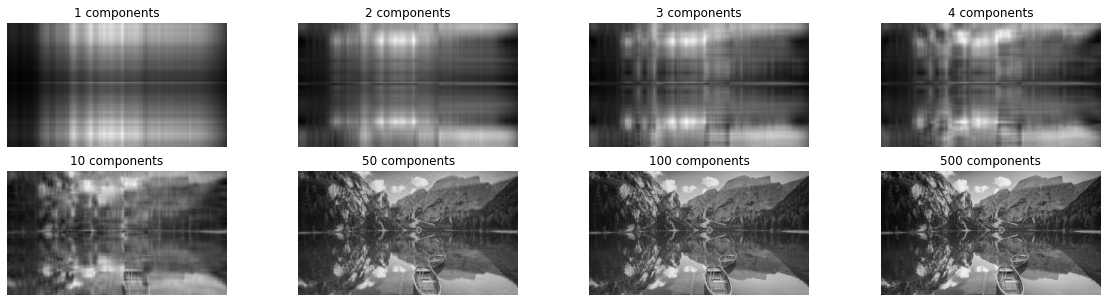
\includegraphics[scale=0.4]{image5.png}
\end{center}

\paragraph{PCA for moving objects tracking on video}

The duration of whole test video images is 108 seconds, and two moving
objects with different sizes (one regular car and one motorcycle) are the main targets in the test. The result of interested clip extraction is shown below. The x axis represents the serial number of the frames and the y axis indicates the number of motion pixels. Two significant peaks can be evidently observed in the graphic, there are two periods that contain moving objects are detected.
\begin{center}
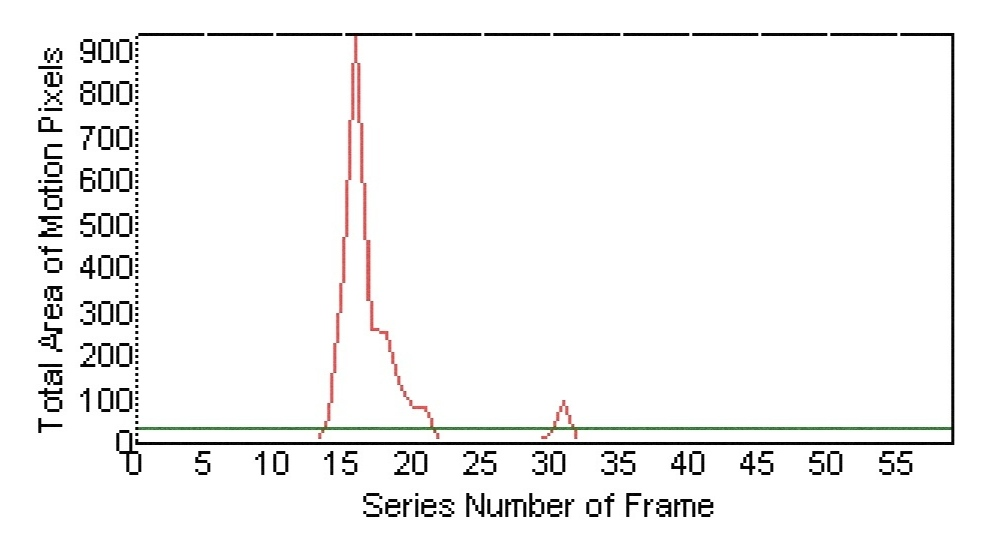
\includegraphics[scale=0.3]{image1.jpg}
\end{center}

The interested clips of two periods are respectively shown in the first picture below (regular car and motorcycle). After extracting the interested clips and converting to PC space, a series of corresponding PC image sequences are revealed in the second picture. 

\begin{center}
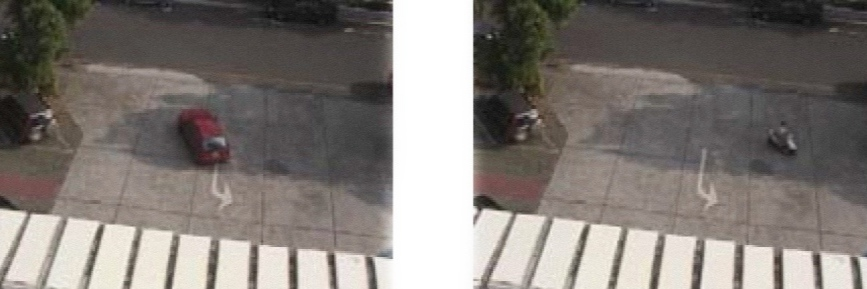
\includegraphics[scale=0.3]{image2.jpg}
\end{center}

\begin{center}
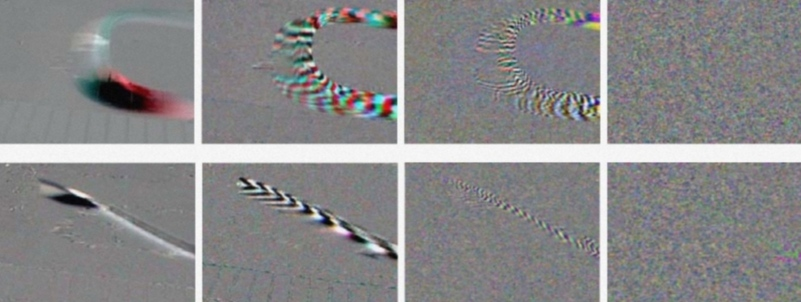
\includegraphics[scale=0.4]{image3.jpg}
\end{center}

















\end{document}

